\documentclass[a4paper, twocolumn, 11pt, oneside]{memoir}
\usepackage{preamble}

\author{Laurits Nikolaj Stokholm\thanks{au568919}}
\title{A brief introduction to \LaTeX documents}
%\subtitle{Numerical approximation of the exponential}
\date{\today}



\begin{document}

\twocolumn[
\maketitle
\begin{onecolabstract}
\noindent
This short paper was written as part of the course \emph{Practical Programming and Numerical
Methods}. Herein, I will introduce the exponential function and show an implementation
of it using the programming language of C. The result is in fine agreement with
both the exponential function as defined in the standard mathematics package
and in the gnuplot tool. Evenmore, we show some basic capabilities of the
\LaTeX system such as the mathematical cross references, sections and including
plots generated by the gnuplot software. The project is handled by the make
utility tool, and a link to the repository can be found
at \url{https://github.com/LauritsStokholm/ppnm}.
\end{onecolabstract}
]

\section{A Bird's eye view}
%\showthe\columnwidth
\subsection{Analysis of real-variables}
From the beginning, the scalar exponential function $\exp: t \rightarrow
exp(a\cdot t)$ draws much of its significance from two very peculiar properties
it enjoys. For one thing, it satisfies the functional equation
\begin{equation}
  f(t+s) = f(t)\cdot f(s). % \nonumber
\label{eq:FE}
\end{equation}
which, in the view of algebraic mappings between groups, gives the group
homomorphism from $\left(\mathbb{R}, +\right)$ to $\left(\mathbb{R}_{>0}, \cdot\right)$, where
$\mathbb{R}_{>0} = \{x\in\mathbb{R} \| x > 0 \}$. Without the exponential
function, this fact would be hidden.

On the other hand, the exponential function satisfies the differential equation
\begin{equation}
  \diff[d]{f}{t} = a\cdot f(t) % \nonumber
\label{eq:DE}
\end{equation}
\cref{eq:FE} is the analogue to the slide rule of logarithms as first used by John
Napier\cite{john_napier_wiki}.
\cref{eq:DE} appears to be of a quite different
nature. Historically developed to expand on the idea that the growth rate of an
amount of money under the influence of continuously calculated compound
interest to be directly proportional at any time to the amount attained at that
time. Leonhard Euler put \cref{eq:FE} and \cref{eq:DE} into a coherent context
showing the series
\begin{align}
  \sum_{n=0}^{\infty} \frac{t^n}{n!} = \lim_{n\rightarrow \infty} \left(1 + \frac{t}{n}\right)^n = \text{e}^t% \nonumber
\label{eq:series}
\end{align}
where we differentiate between the function $\exp$ and the irrational number
$e$.
\cref{eq:series} is what extends the exponential function to almost any other
field of mathematics. It is the basis of Eulers identity, which easily extends
the exponential function to complex variables; and in fact to operator calculus
and functional analysis.
Irrefutably vital without exception for the entire field of mathematics and
thus also of the natural sciences.

\section{Numerical Implementation}
In this section a numerical implemtation of the exponential function will be
described. Here, we take ground in the series expansion of \cref{eq:series}.
A naive method would be to hard code a finite degree polynomial estimation of
the series expansion. This would lead to the following downsides and
considerations:
\begin{itemize}
  \item Each term varies in size exponentially and thus as the total sum is
    computed in sequence from left to right, a numerical error is introduced.
  \item A large number of functional operations will surely be called, unless
    an explicit consideration to this is written.
    For instance, instead of utilising the power function for
    each term, one can reduce this number by isolating a common factor out.
  \item Even further, using the quicker multiplication operator instead of the
    power function, compilation time will be lowered.
  \item Since the series expansion will be estimated by a finite sum, then for
    large values of the argument, the series approximation will diverge from
    the exact series expansion.
  \item In case of a negative argument, every uneven term will be negative, and
    and thus another source of error is introduced by adding positive and
    negative terms.

\end{itemize}
Luckily, these considerations are not too tedious. There exists a
``quick-and-dirty" method to estimate the series expansion \cref{eq:series};
giving a numerical implementation of the exponential function. This is given in
\cref{fig:code}. First of all, the terms are monotonically increasing, so the addition
is less error prone. Secondly, there is defined a handler for relatively large
values of the argument, such that the series expansion is always for small
arguments. Lastly, for negative values the addition is summed using strictly
positive terms.
\cref{eq:series}.
\begin{figure}[ht]
\begin{lstlisting}[language=c]
double my_exp(double x)
{
if (x<0) return 1/my_exp(-x);
if (x>1./8) return pow(my_exp(x/2),2);
return 1+x*\
(1+x/2*(1+x/3*(1+x/4*(1+x/5*\
(1+x/6*(1+x/7*(1+x/8*(1+x/9*\
(1+x/10)))))))));
}
\end{lstlisting}
\caption{Explicit code for implementation of the exponential function.}
\label{fig:code}
\end{figure}

\begin{figure}[ht]
\centering
% GNUPLOT: LaTeX picture with Postscript
\begingroup
\bfseries 
  \makeatletter
  \providecommand\color[2][]{%
    \GenericError{(gnuplot) \space\space\space\@spaces}{%
      Package color not loaded in conjunction with
      terminal option `colourtext'%
    }{See the gnuplot documentation for explanation.%
    }{Either use 'blacktext' in gnuplot or load the package
      color.sty in LaTeX.}%
    \renewcommand\color[2][]{}%
  }%
  \providecommand\includegraphics[2][]{%
    \GenericError{(gnuplot) \space\space\space\@spaces}{%
      Package graphicx or graphics not loaded%
    }{See the gnuplot documentation for explanation.%
    }{The gnuplot epslatex terminal needs graphicx.sty or graphics.sty.}%
    \renewcommand\includegraphics[2][]{}%
  }%
  \providecommand\rotatebox[2]{#2}%
  \@ifundefined{ifGPcolor}{%
    \newif\ifGPcolor
    \GPcolortrue
  }{}%
  \@ifundefined{ifGPblacktext}{%
    \newif\ifGPblacktext
    \GPblacktexttrue
  }{}%
  % define a \g@addto@macro without @ in the name:
  \let\gplgaddtomacro\g@addto@macro
  % define empty templates for all commands taking text:
  \gdef\gplbacktext{}%
  \gdef\gplfronttext{}%
  \makeatother
  \ifGPblacktext
    % no textcolor at all
    \def\colorrgb#1{}%
    \def\colorgray#1{}%
  \else
    % gray or color?
    \ifGPcolor
      \def\colorrgb#1{\color[rgb]{#1}}%
      \def\colorgray#1{\color[gray]{#1}}%
      \expandafter\def\csname LTw\endcsname{\color{white}}%
      \expandafter\def\csname LTb\endcsname{\color{black}}%
      \expandafter\def\csname LTa\endcsname{\color{black}}%
      \expandafter\def\csname LT0\endcsname{\color[rgb]{1,0,0}}%
      \expandafter\def\csname LT1\endcsname{\color[rgb]{0,1,0}}%
      \expandafter\def\csname LT2\endcsname{\color[rgb]{0,0,1}}%
      \expandafter\def\csname LT3\endcsname{\color[rgb]{1,0,1}}%
      \expandafter\def\csname LT4\endcsname{\color[rgb]{0,1,1}}%
      \expandafter\def\csname LT5\endcsname{\color[rgb]{1,1,0}}%
      \expandafter\def\csname LT6\endcsname{\color[rgb]{0,0,0}}%
      \expandafter\def\csname LT7\endcsname{\color[rgb]{1,0.3,0}}%
      \expandafter\def\csname LT8\endcsname{\color[rgb]{0.5,0.5,0.5}}%
    \else
      % gray
      \def\colorrgb#1{\color{black}}%
      \def\colorgray#1{\color[gray]{#1}}%
      \expandafter\def\csname LTw\endcsname{\color{white}}%
      \expandafter\def\csname LTb\endcsname{\color{black}}%
      \expandafter\def\csname LTa\endcsname{\color{black}}%
      \expandafter\def\csname LT0\endcsname{\color{black}}%
      \expandafter\def\csname LT1\endcsname{\color{black}}%
      \expandafter\def\csname LT2\endcsname{\color{black}}%
      \expandafter\def\csname LT3\endcsname{\color{black}}%
      \expandafter\def\csname LT4\endcsname{\color{black}}%
      \expandafter\def\csname LT5\endcsname{\color{black}}%
      \expandafter\def\csname LT6\endcsname{\color{black}}%
      \expandafter\def\csname LT7\endcsname{\color{black}}%
      \expandafter\def\csname LT8\endcsname{\color{black}}%
    \fi
  \fi
    \setlength{\unitlength}{0.0500bp}%
    \ifx\gptboxheight\undefined%
      \newlength{\gptboxheight}%
      \newlength{\gptboxwidth}%
      \newsavebox{\gptboxtext}%
    \fi%
    \setlength{\fboxrule}{0.5pt}%
    \setlength{\fboxsep}{1pt}%
\begin{picture}(4380.00,4380.00)%
      \csname LTb\endcsname%%
      \put(2190,4157){\makebox(0,0){\strut{}Implementation of exponential function}}%
    \gplgaddtomacro\gplbacktext{%
      \csname LTb\endcsname%%
      \put(854,2190){\makebox(0,0)[r]{\strut{}$0$}}%
      \csname LTb\endcsname%%
      \put(854,2408){\makebox(0,0)[r]{\strut{}$20$}}%
      \csname LTb\endcsname%%
      \put(854,2626){\makebox(0,0)[r]{\strut{}$40$}}%
      \csname LTb\endcsname%%
      \put(854,2844){\makebox(0,0)[r]{\strut{}$60$}}%
      \csname LTb\endcsname%%
      \put(854,3062){\makebox(0,0)[r]{\strut{}$80$}}%
      \csname LTb\endcsname%%
      \put(854,3279){\makebox(0,0)[r]{\strut{}$100$}}%
      \csname LTb\endcsname%%
      \put(854,3497){\makebox(0,0)[r]{\strut{}$120$}}%
      \csname LTb\endcsname%%
      \put(854,3715){\makebox(0,0)[r]{\strut{}$140$}}%
      \csname LTb\endcsname%%
      \put(854,3933){\makebox(0,0)[r]{\strut{}$160$}}%
    }%
    \gplgaddtomacro\gplfronttext{%
      \csname LTb\endcsname%%
      \put(285,3061){\rotatebox{-270}{\makebox(0,0){\strut{}y}}}%
      \csname LTb\endcsname%%
      \put(2372,1968){\makebox(0,0){\strut{}x}}%
      \csname LTb\endcsname%%
      \put(2826,3732){\makebox(0,0)[r]{\strut{}self-implemented}}%
      \csname LTb\endcsname%%
      \put(2826,3509){\makebox(0,0)[r]{\strut{}math.h}}%
      \csname LTb\endcsname%%
      \put(2826,3286){\makebox(0,0)[r]{\strut{}gnuplot}}%
    }%
    \gplgaddtomacro\gplbacktext{%
      \csname LTb\endcsname%%
      \put(854,892){\makebox(0,0)[r]{\strut{}$-1$}}%
      \csname LTb\endcsname%%
      \put(854,1161){\makebox(0,0)[r]{\strut{}$-0.5$}}%
      \csname LTb\endcsname%%
      \put(854,1429){\makebox(0,0)[r]{\strut{}$0$}}%
      \csname LTb\endcsname%%
      \put(854,1698){\makebox(0,0)[r]{\strut{}$0.5$}}%
      \csname LTb\endcsname%%
      \put(854,1966){\makebox(0,0)[r]{\strut{}$1$}}%
      \csname LTb\endcsname%%
      \put(976,669){\makebox(0,0){\strut{}$-2$}}%
      \csname LTb\endcsname%%
      \put(1375,669){\makebox(0,0){\strut{}$-1$}}%
      \csname LTb\endcsname%%
      \put(1774,669){\makebox(0,0){\strut{}$0$}}%
      \csname LTb\endcsname%%
      \put(2173,669){\makebox(0,0){\strut{}$1$}}%
      \csname LTb\endcsname%%
      \put(2572,669){\makebox(0,0){\strut{}$2$}}%
      \csname LTb\endcsname%%
      \put(2971,669){\makebox(0,0){\strut{}$3$}}%
      \csname LTb\endcsname%%
      \put(3370,669){\makebox(0,0){\strut{}$4$}}%
      \csname LTb\endcsname%%
      \put(3769,669){\makebox(0,0){\strut{}$5$}}%
    }%
    \gplgaddtomacro\gplfronttext{%
      \csname LTb\endcsname%%
      \put(163,1429){\rotatebox{-270}{\makebox(0,0){\strut{}y}}}%
      \csname LTb\endcsname%%
      \put(2372,335){\makebox(0,0){\strut{}x}}%
      \csname LTb\endcsname%%
      \put(2826,1765){\makebox(0,0)[r]{\strut{}Residual}}%
    }%
    \gplbacktext
    \put(0,0){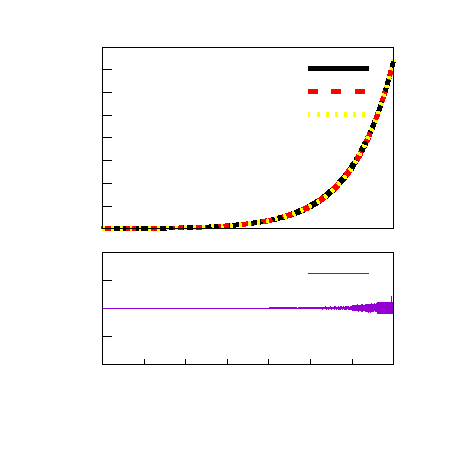
\includegraphics{exp}}%
    \gplfronttext
  \end{picture}%
\endgroup

\caption{A comparison of the exponential function defined by the header
\textsl{math.h}, in the plotting tool \textsl{gnuplot} and as defined in this
paper implementation.}
\label{fig:exp.tex}
\end{figure}

\section{Conclusion}
The residuals of this quick and dirty implementation compared to the
exponential function given in the mathematical header \textsl{math.h} is of the
order of $10^{-12}$ which compared to the precision of a double (15 decimals)
is very good. The cutoff at the 10th term was arbitrary, and one could of
course consider a higher degree polynomial estimation. All in all, we
can conclude a successfull implementation of the exponential function.

\printbibliography

\end{document}
